
\documentclass[12pt,a4paper]{article}
\usepackage[utf8]{inputenc}
\usepackage[T1]{fontenc}
\usepackage{geometry}
\usepackage{setspace}
\usepackage{hyperref}
\usepackage{enumitem}
\usepackage{booktabs}
\usepackage{longtable}
\usepackage{xcolor}
\usepackage{caption}
\usepackage{tikz}
\usetikzlibrary{arrows.meta,positioning,shapes.geometric,shapes.misc,calc}
\geometry{margin=1in}
\setstretch{1.2}
\hypersetup{colorlinks=true,linkcolor=blue,urlcolor=blue}

% TikZ styles
\tikzset{
  actor/.style={draw, thick, fill=white, minimum width=10mm, minimum height=22mm, rounded corners=1mm},
  usecase/.style={draw, ellipse, align=center, minimum width=24mm, minimum height=8mm, font=\small, fill=white},
  lifeline/.style={draw, thick, fill=white, minimum width=30mm, minimum height=8mm},
  message/.style={-Latex, thick},
  activation/.style={fill=black!10, minimum width=3mm},
}

\title{\textbf{The Chattala}\\\large Use Case \& Sequence Diagram Report}
\author{Prepared for: ARIFUR RAHMAN}
\date{\today}

\begin{document}
\maketitle
\tableofcontents
\newpage

\section{System Overview}
\textit{The Chattala} is a web platform for the Chattogram community that unifies: (i) community Q\&A (ask, answer, accept), (ii) civic issue reporting with basic moderation and status tracking, (iii) an archive of authentic content (heritage/culture/tourism), (iv) a digital marketplace with a 24-hour fulfilment commitment, and (v) a lightweight rewards program. The MVP runs on PHP (XAMPP) + MySQL with a Bootstrap UI and session-based authentication.

\section{Actors}
\begin{longtable}{@{}p{0.24\linewidth}p{0.70\linewidth}@{}}
\toprule
\textbf{Actor} & \textbf{Description} \\
\midrule
Resident (Verified User) & Primary end-user: asks/answers questions, reports issues, reads the archive, buys marketplace items, and redeems rewards. \\
Moderator & Curates content, handles flags, and updates civic issue statuses. \\
Admin & Manages categories/taxonomies, user roles, configurations, and metrics. \\
Vendor & Maintains product catalog and fulfils digital orders within 24 hours. \\
Payment Gateway (optional) & External service to authorise/capture payments in future phases. \\
Email/SMS Provider (optional) & Delivers notifications (order confirmations, redemption updates). \\
\bottomrule
\end{longtable}

\section{Use Case Diagram}
\begin{figure}[h]
\centering
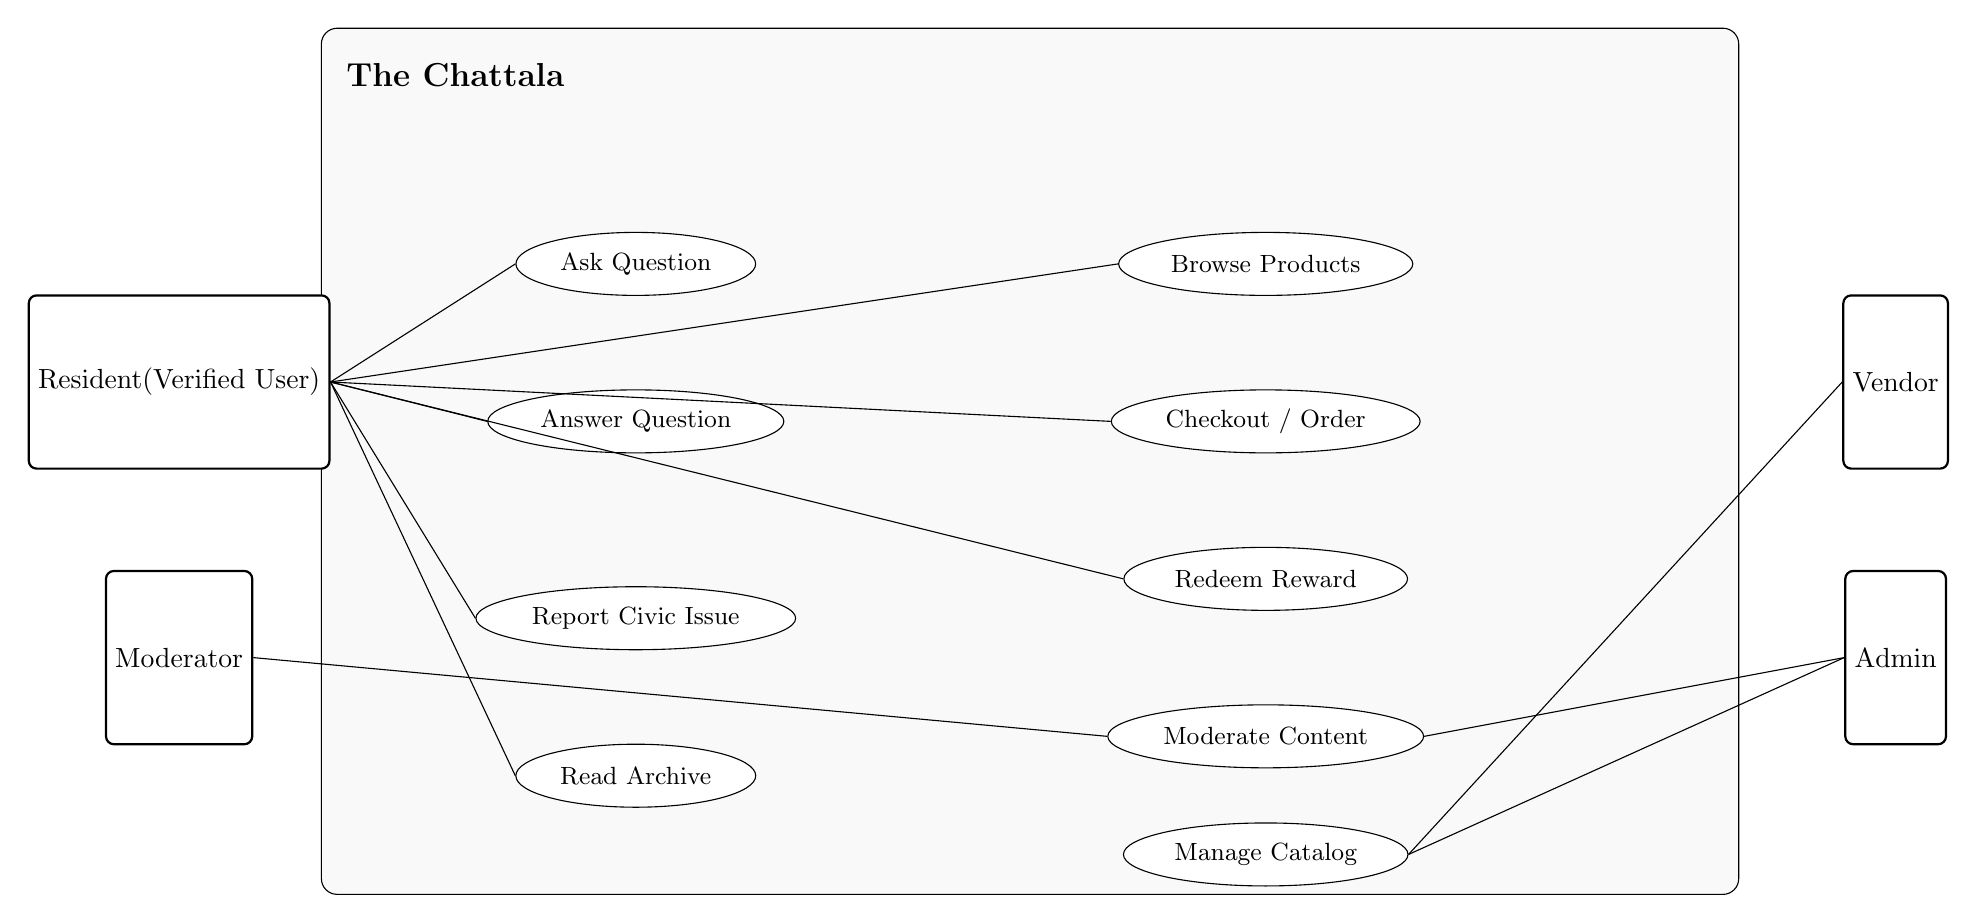
\begin{tikzpicture}[x=1mm,y=1mm]
  % System boundary
  \node[draw, rounded corners=2mm, minimum width=180mm, minimum height=110mm, anchor=north west, fill=gray!5] (sys) at (0,0) {};
  \node[anchor=west] at (2, -6) {\large \textbf{The Chattala}};

  % Actors
  \node[actor] (resident) at (-18,-45) {Resident\\(Verified User)};
  \node[actor] (moderator) at (-18,-80) {Moderator};
  \node[actor] (vendor)    at (200,-45) {Vendor};
  \node[actor] (admin)     at (200,-80) {Admin};

  % Use cases (left cluster: community)
  \node[usecase] (ask)   at (40,-30) {Ask Question};
  \node[usecase] (ans)   at (40,-50) {Answer Question};
  \node[usecase] (issue) at (40,-75) {Report Civic Issue};
  \node[usecase] (read)  at (40,-95) {Read Archive};

  % Use cases (right cluster: commerce + admin)
  \node[usecase] (browse)   at (120,-30) {Browse Products};
  \node[usecase] (checkout) at (120,-50) {Checkout / Order};
  \node[usecase] (redeem)   at (120,-70) {Redeem Reward};
  \node[usecase] (moderate) at (120,-90) {Moderate Content};
  \node[usecase] (catalog)  at (120,-105) {Manage Catalog};

  % Associations
  \draw (resident.east) -- (ask.west);
  \draw (resident.east) -- (ans.west);
  \draw (resident.east) -- (issue.west);
  \draw (resident.east) -- (read.west);
  \draw (resident.east) -- (browse.west);
  \draw (resident.east) -- (checkout.west);
  \draw (resident.east) -- (redeem.west);

  \draw (moderator.east) -- (moderate.west);
  \draw (admin.west) -- (moderate.east);
  \draw (vendor.west) -- (catalog.east);
  \draw (admin.west) -- (catalog.east);
\end{tikzpicture}
\caption{Use Case Diagram for The Chattala}
\end{figure}

\clearpage
\section{Textual Use Case Specifications}
\subsection*{UC-Q1: Ask Question}
\textbf{Primary Actor:} Resident\\
\textbf{Goal:} Submit a new question with title and body.\\
\textbf{Pre-conditions:} Authenticated Resident; DB reachable.\\
\textbf{Post-conditions:} Question stored; visible in the list; author = current user.\\
\textbf{Main Flow:}
\begin{enumerate}[leftmargin=*]
  \item Resident opens \emph{Ask Question}.
  \item System shows form (title, body).
  \item Resident submits; System validates; inserts the record.
  \item System redirects to Question Details.
\end{enumerate}
\textbf{Alternates/Exceptions:} Validation or DB error \(\to\) show friendly error and log.

\subsection*{UC-Q2: Answer Question}
\textbf{Primary Actor:} Resident\\
\textbf{Main Flow:} Open a question \(\to\) submit an answer \(\to\) system validates and inserts \(\to\) page refreshes with the new answer.

\subsection*{UC-Q3: Mark Accepted Answer (optional)}
\textbf{Primary Actor:} Resident (author)\\
\textbf{Main Flow:} Select an answer as accepted; system marks \texttt{is\_accepted=true}.

\subsection*{UC-I1: Report Civic Issue}
\textbf{Primary Actor:} Resident\\
\textbf{Main Flow:} Open form \(\to\) submit title/description/location \(optional\) \(\to\) system inserts with status=Open.

\subsection*{UC-I2: Update Issue Status}
\textbf{Primary Actor:} Moderator\\
\textbf{Main Flow:} Open issue \(\to\) set status: Open \(\to\) In Review \(\to\) Resolved/Closed.

\subsection*{UC-A1: Read Archive}\textbf{ Primary Actor:} Resident. Browse categories; open article details.

\subsection*{UC-M1: Browse Products}\textbf{ Primary Actor:} Resident. View active products with price.

\subsection*{UC-M2: Checkout / Order}
\textbf{Primary Actor:} Resident\\
\textbf{Main Flow:} Select product \(\to\) Buy Now \(\to\) System creates Order+Items (demo Paid) \(\to\) show confirmation/history.

\subsection*{UC-R1: Redeem Reward}
\textbf{Primary Actor:} Resident\\
\textbf{Main Flow:} Open rewards \(\to\) redeem \(\to\) system creates Pending redemption \(admin processes later\).

\subsection*{UC-C1: Moderate Content}\textbf{ Primary Actor:} Moderator/Admin. Review and hide/remove content.

\subsection*{UC-C2: Manage Catalog}\textbf{ Primary Actor:} Vendor/Admin. Create/update products.

\clearpage
\section{Sequence Diagrams}

\subsection{SD-Q: Ask a Question (Happy Path)}
\begin{figure}[h]
\centering
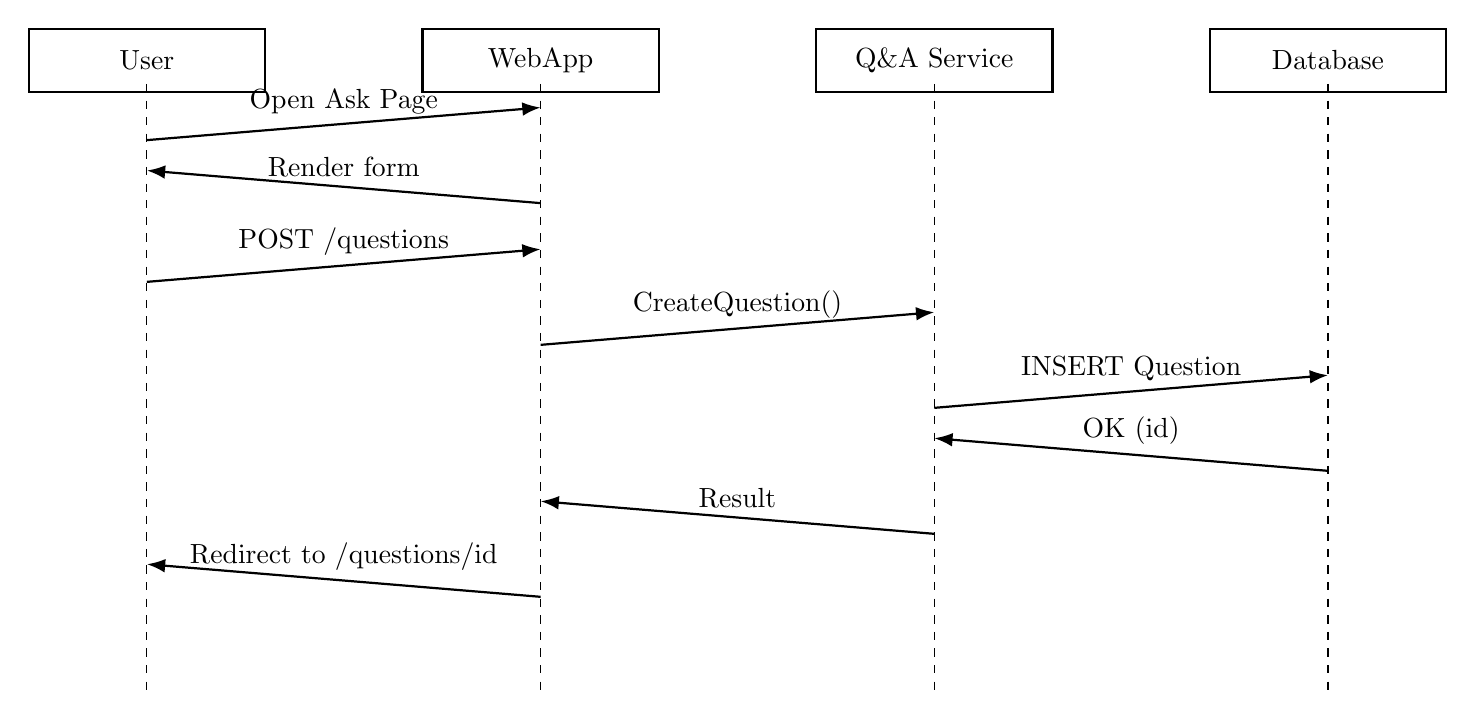
\begin{tikzpicture}[x=1mm,y=1mm]
  % Lifelines
  \node[lifeline] (user) at (0,0) {User};
  \node[lifeline] (web) at (50,0) {WebApp};
  \node[lifeline] (svc) at (100,0) {Q\&A Service};
  \node[lifeline] (db)  at (150,0) {Database};
  % Vertical dashed lifelines
  \foreach \x in {0,50,100,150} {\draw[dashed] (\x,-3) -- (\x,-80);}
  % Messages
  \draw[message] (user.south)++(0,-6) -- node[above]{Open Ask Page} (web.south|-0,-6);
  \draw[message] (web.south)++(0,-14) -- node[above]{Render form} (user.south|-0,-14);
  \draw[message] (user.south)++(0,-24) -- node[above]{POST /questions} (web.south|-0,-24);
  \draw[message] (web.south)++(0,-32) -- node[above]{CreateQuestion()} (svc.south|-0,-32);
  \draw[message] (svc.south)++(0,-40) -- node[above]{INSERT Question} (db.south|-0,-40);
  \draw[message] (db.south)++(0,-48) -- node[above]{OK (id)} (svc.south|-0,-48);
  \draw[message] (svc.south)++(0,-56) -- node[above]{Result} (web.south|-0,-56);
  \draw[message] (web.south)++(0,-64) -- node[above]{Redirect to /questions/{id}} (user.south|-0,-64);
\end{tikzpicture}
\caption{Sequence: Ask a Question}
\end{figure}

\subsection{SD-I: Report Issue \& Moderator Resolves}
\begin{figure}[h]
\centering
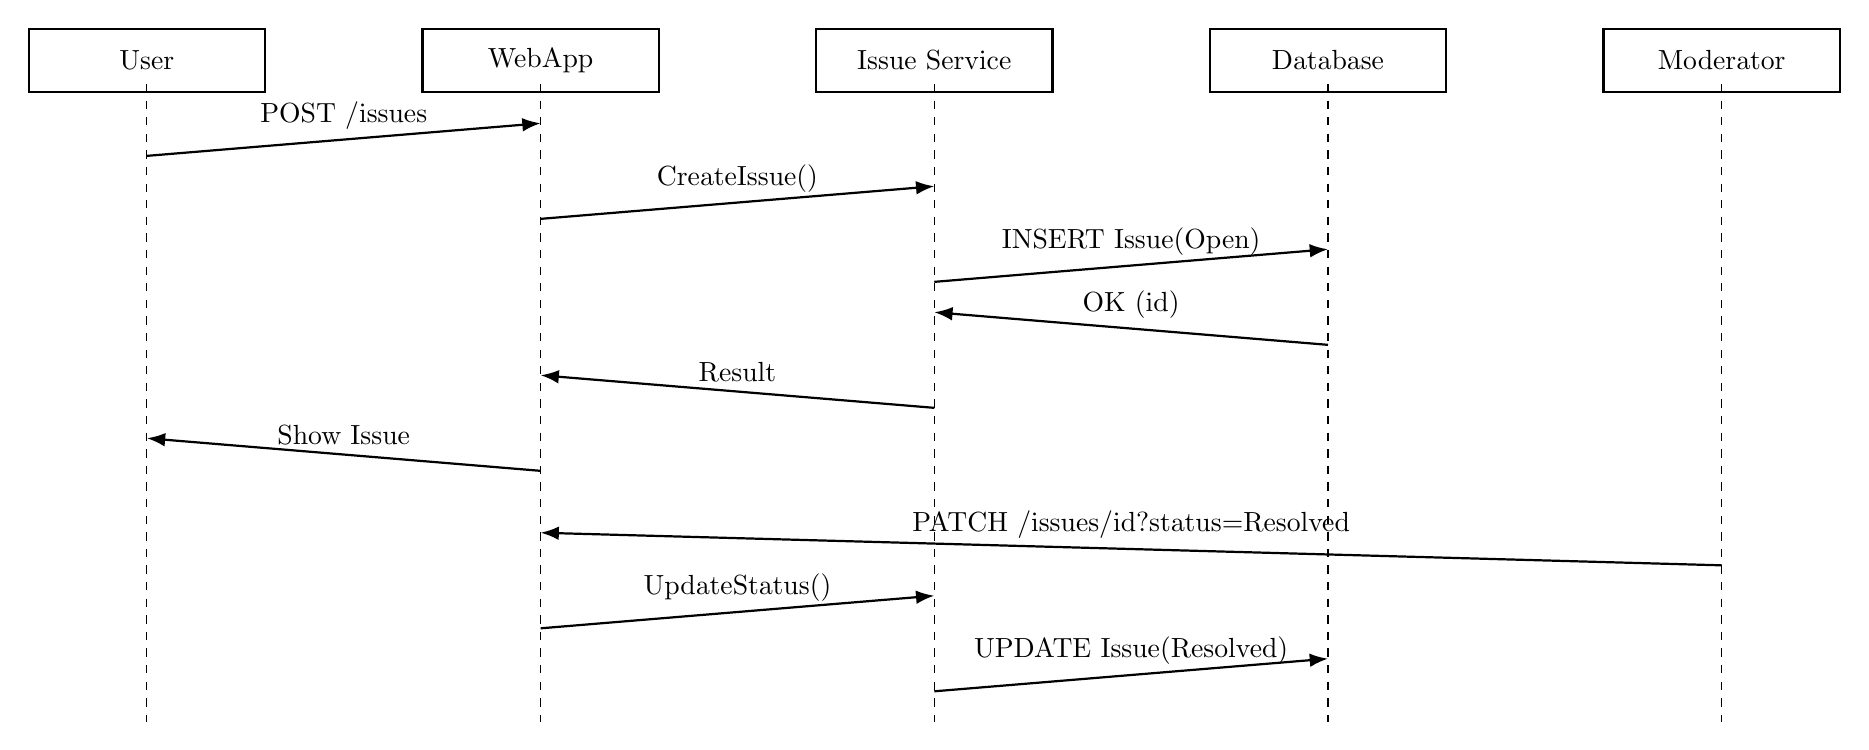
\begin{tikzpicture}[x=1mm,y=1mm]
  \node[lifeline] (user) at (0,0) {User};
  \node[lifeline] (web) at (50,0) {WebApp};
  \node[lifeline] (issue) at (100,0) {Issue Service};
  \node[lifeline] (db)  at (150,0) {Database};
  \foreach \x in {0,50,100,150} {\draw[dashed] (\x,-3) -- (\x,-84);}
  \draw[message] (user.south)++(0,-8) -- node[above]{POST /issues} (web.south|-0,-8);
  \draw[message] (web.south)++(0,-16) -- node[above]{CreateIssue()} (issue.south|-0,-16);
  \draw[message] (issue.south)++(0,-24) -- node[above]{INSERT Issue(Open)} (db.south|-0,-24);
  \draw[message] (db.south)++(0,-32) -- node[above]{OK (id)} (issue.south|-0,-32);
  \draw[message] (issue.south)++(0,-40) -- node[above]{Result} (web.south|-0,-40);
  \draw[message] (web.south)++(0,-48) -- node[above]{Show Issue} (user.south|-0,-48);
  % Moderator phase
  \node[lifeline] (mod) at (200,0) {Moderator};
  \draw[dashed] (200,-3) -- (200,-84);
  \draw[message] (mod.south)++(0,-60) -- node[above]{PATCH /issues/{id}?status=Resolved} (web.south|-0,-60);
  \draw[message] (web.south)++(0,-68) -- node[above]{UpdateStatus()} (issue.south|-0,-68);
  \draw[message] (issue.south)++(0,-76) -- node[above]{UPDATE Issue(Resolved)} (db.south|-0,-76);
\end{tikzpicture}
\caption{Sequence: Report Issue and Resolve}
\end{figure}

\subsection{SD-M: Checkout \& 24h Fulfilment (Simplified)}
\begin{figure}[h]
\centering
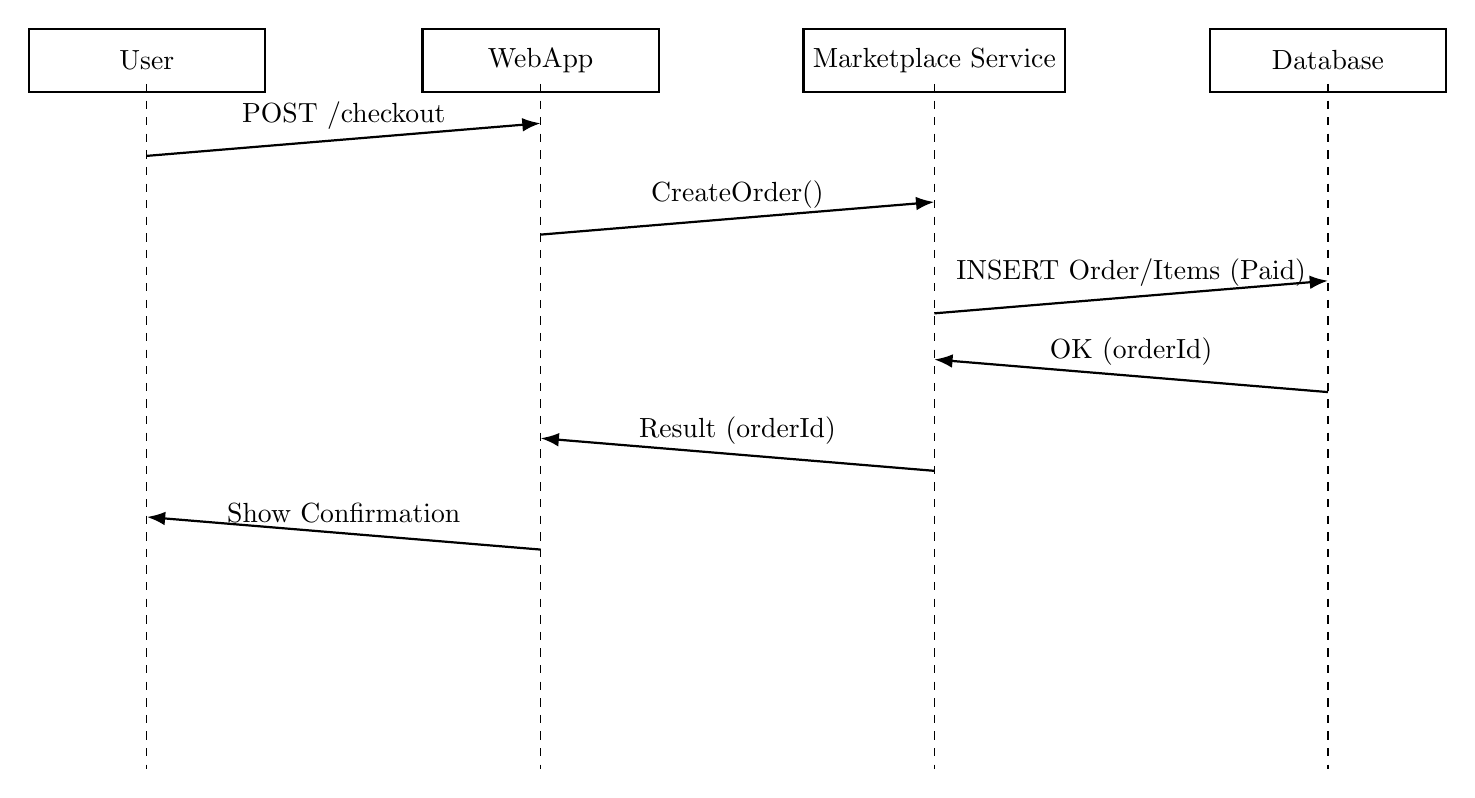
\begin{tikzpicture}[x=1mm,y=1mm]
  \node[lifeline] (user) at (0,0) {User};
  \node[lifeline] (web) at (50,0) {WebApp};
  \node[lifeline] (mkt) at (100,0) {Marketplace Service};
  \node[lifeline] (db)  at (150,0) {Database};
  \foreach \x in {0,50,100,150} {\draw[dashed] (\x,-3) -- (\x,-90);}
  \draw[message] (user.south)++(0,-8) -- node[above]{POST /checkout} (web.south|-0,-8);
  \draw[message] (web.south)++(0,-18) -- node[above]{CreateOrder()} (mkt.south|-0,-18);
  \draw[message] (mkt.south)++(0,-28) -- node[above]{INSERT Order/Items (Paid)} (db.south|-0,-28);
  \draw[message] (db.south)++(0,-38) -- node[above]{OK (orderId)} (mkt.south|-0,-38);
  \draw[message] (mkt.south)++(0,-48) -- node[above]{Result (orderId)} (web.south|-0,-48);
  \draw[message] (web.south)++(0,-58) -- node[above]{Show Confirmation} (user.south|-0,-58);
\end{tikzpicture}
\caption{Sequence: Checkout (MVP without PG)}
\end{figure}

\paragraph{Future with Payment Gateway} Authorise amount before persisting the order; capture funds post-fulfilment; persist status timeline; handle failure callbacks.

\clearpage
\section{Design Notes \& Constraints}
Runtime: XAMPP (Apache/PHP/MySQL), session auth, PDO prepared statements. Security (Phase-1): bcrypt password hashing on registration, server-side validation, add CSRF tokens. Responsive Bootstrap UI, clear form errors. Use pagination for large lists; consider caching. Logs for errors and simple counters for admin.

\section{Traceability (Use Cases \textrightarrow{} Modules)}
\begin{longtable}{@{}p{0.30\linewidth}p{0.60\linewidth}@{}}
\toprule
\textbf{Module} & \textbf{Key Use Cases} \\
\midrule
Q\&A & UC-Q1, UC-Q2, UC-Q3 \\
Civic Issues & UC-I1, UC-I2 \\
Archive & UC-A1 \\
Marketplace & UC-M1, UC-M2 \\
Rewards & UC-R1 \\
Moderation/Catalog & UC-C1, UC-C2 \\
\bottomrule
\end{longtable}

\end{document}
